\section{Logbook reports: Exploits in Planika Jama}

   \fullwidthbox{Day 4 - Tuesday - Planika (Team JJ)}{
                    Rigged down the end of the rift and 1st Pitch in \passage{Planika}.
Pleasant surprise in the first chamber. The snow slope was quite melted
next to the pitch wall, so we were able to go all the way down. We
noticed a way on and started smashing the ice wall, feeling the draught.
We manage to get through, but after few meter it choked again with the
ice coming very close to wall. Back on the snow slope. On top we noticed
that another meltwater pit leading to the bottom of the ice, but this
needed bolting to get down, so we decided to continue the way. But not
for long, because a lot of fresh snow blocked the way forward. After
digging a bit through it we decided that a different route would yield a
way on. We were very cold as well.

Back on the surface, there was still time for me to chop down and
prepare some wood for the fire. Jarv walked down to Ravne to carry some
more stuff up.     \name{Jana Čarga} }

\margininbox{Planika Jama}{
     \begin{itemize}
    \item Jana Čarga
    \item Jarvist Frost
    \item James "Tetley" Hooper
    \end{itemize}}{\explo}

\subsection{24.07.08 - Finding Echo Rift}

Went down and bolt in the first snow chamber to go down the new way,
where the snow has melted. \textasciitilde 8 m down in the snow tube
hole. The way on was squizy[sic] and tight, but a lot of draught blew in our
faces. We ran out of rope and bolts, so the lead it is still going,
albeit a bit tight.

We surveyed the new cave on the way out: we had gained 24 m of depth. We
still needed to go back and check the original pushing front from 2007,
which was a cold snow chamber.

\tweet{12:00PM Jul 24th, 2008}{Planika: pushed via P8 through snow to tight rift leading to icy P8 with unpushed blow rift on. Now 30m from mona, but offset. 50m deep.}

We had almost finished rigging when we heard: ``Is the rope free?'' It
was Tetley - he had finally come down to \passage{Planika}. He wanted to
head down and take a look at the new going lead. We mentioned to him
that it was tight, which he shrugged off with a ``yeah, yeah\ldots{}''.
He still got stuck in the first rift further down. Not managing to
wrestle free immediately, he lit up a cigarette and started smoking it.
:) On the way out we derigged the yellow \passage{Planika} ropes, to provide the
necessary lengths to rig down to \passage{Monatip} entrance.

\name{Jana Čarga}

\begin{marginfigure}
\checkoddpage \ifoddpage \forcerectofloat \else \forceversofloat \fi
\centering
 \frame{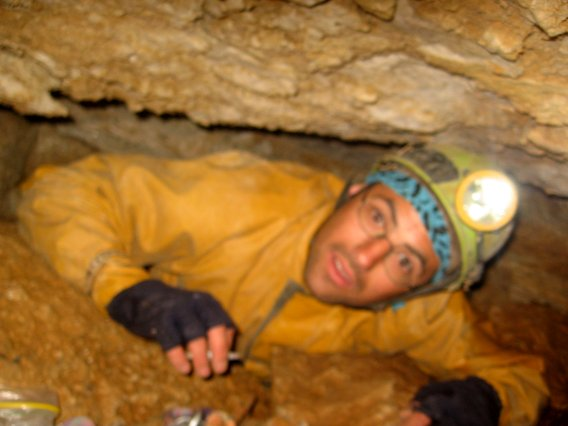
\includegraphics[width=\linewidth]{2008/planika/Jarvist Frost - canon a520 - planika - tet smoking in chest squeeze--orig.jpg}} 
 \caption{Tetley takes a moment in \protect\passage{Planika Jama}'s squeeze. \pic{Jarvist Frost}}
 \label{Tet planika smoke}
\end{marginfigure}


Dropped new melted pitch. Safe rock → awful rope rub. Meh. 1 bolt \&
down, comedy sling backup \& pitch rope stretched across. Pushed to
tight chest-wide rift; ice everywhere. Tight rift meandered to
pitchhead. Located natural hang while Jana fetched survey kit \& rope. 1
dodgy thread \& down. Long sling to stretch out rope ($\approx$ 8
m). This proved troublesome on the way up.

Dropped onto ice-floored
chamber with semi-tight rift off it. 1.5 m diameter hole to small chamber 4
m below. Even tighter rift in same direction from here. Surveyed out
carefully.

Just the otherside of the chest squeeze, Tetley shouted down, having
taken the hyper death slide across the snow. He tried the chest squeeze,
got wedged \& so cracked out his smoke kit \& had a tab.

\name{Jarvist Frost}

\subsection{26.07.08 - Rerigging and pushing}

 \margininbox{Planika Jama}{
     \begin{itemize}
    \item Jarvist Frost
    \item Clewin Griffiths
    \end{itemize}}{\explo}

Ill fated trip! The rerig slowed us down. Clew placed a Y-hang bolt -
went a bit deep, no matter - ``I have a cunning plan''. Wedging a spare
cone lightly into the spit, he protected the thread while cleaning
around. Of course, it didn't come out again. Then he hit a super tight
Alpine-butterfly just 1 m shy of the rebelay. 20 minutes of effort, to
prussic up \& have Jarv gnaw it open. \bignote{Then he lost his knife in a
crevasse} \& spent 20 thoroughly cold minutes digging it out, while Jarv
placed the backup bolt (nice white soft rock). Expanded the chest
squeeze \& finally reached the pushing front rather late. Clew expanded
the pre-pitch squeeze while Jarv rerigged \& then attempted the higher,
better rift.

Rift: Phreatic top slightly less than body crawl sized tube, less than
chest width vadose. But transition zone is very friable. I got
$\approx$ 3 m in, to see 2 m rift → chamber. Drafting \emph{IN}.
Chamber has fist sized boulders in it. Turns right.

GOING!!! ( with instrument of destruction)

\name{Jarvist Frost}


\begin{pagefigure}
\checkoddpage \ifoddpage \forcerectofloat \else \forceversofloat \fi
\centering
\frame{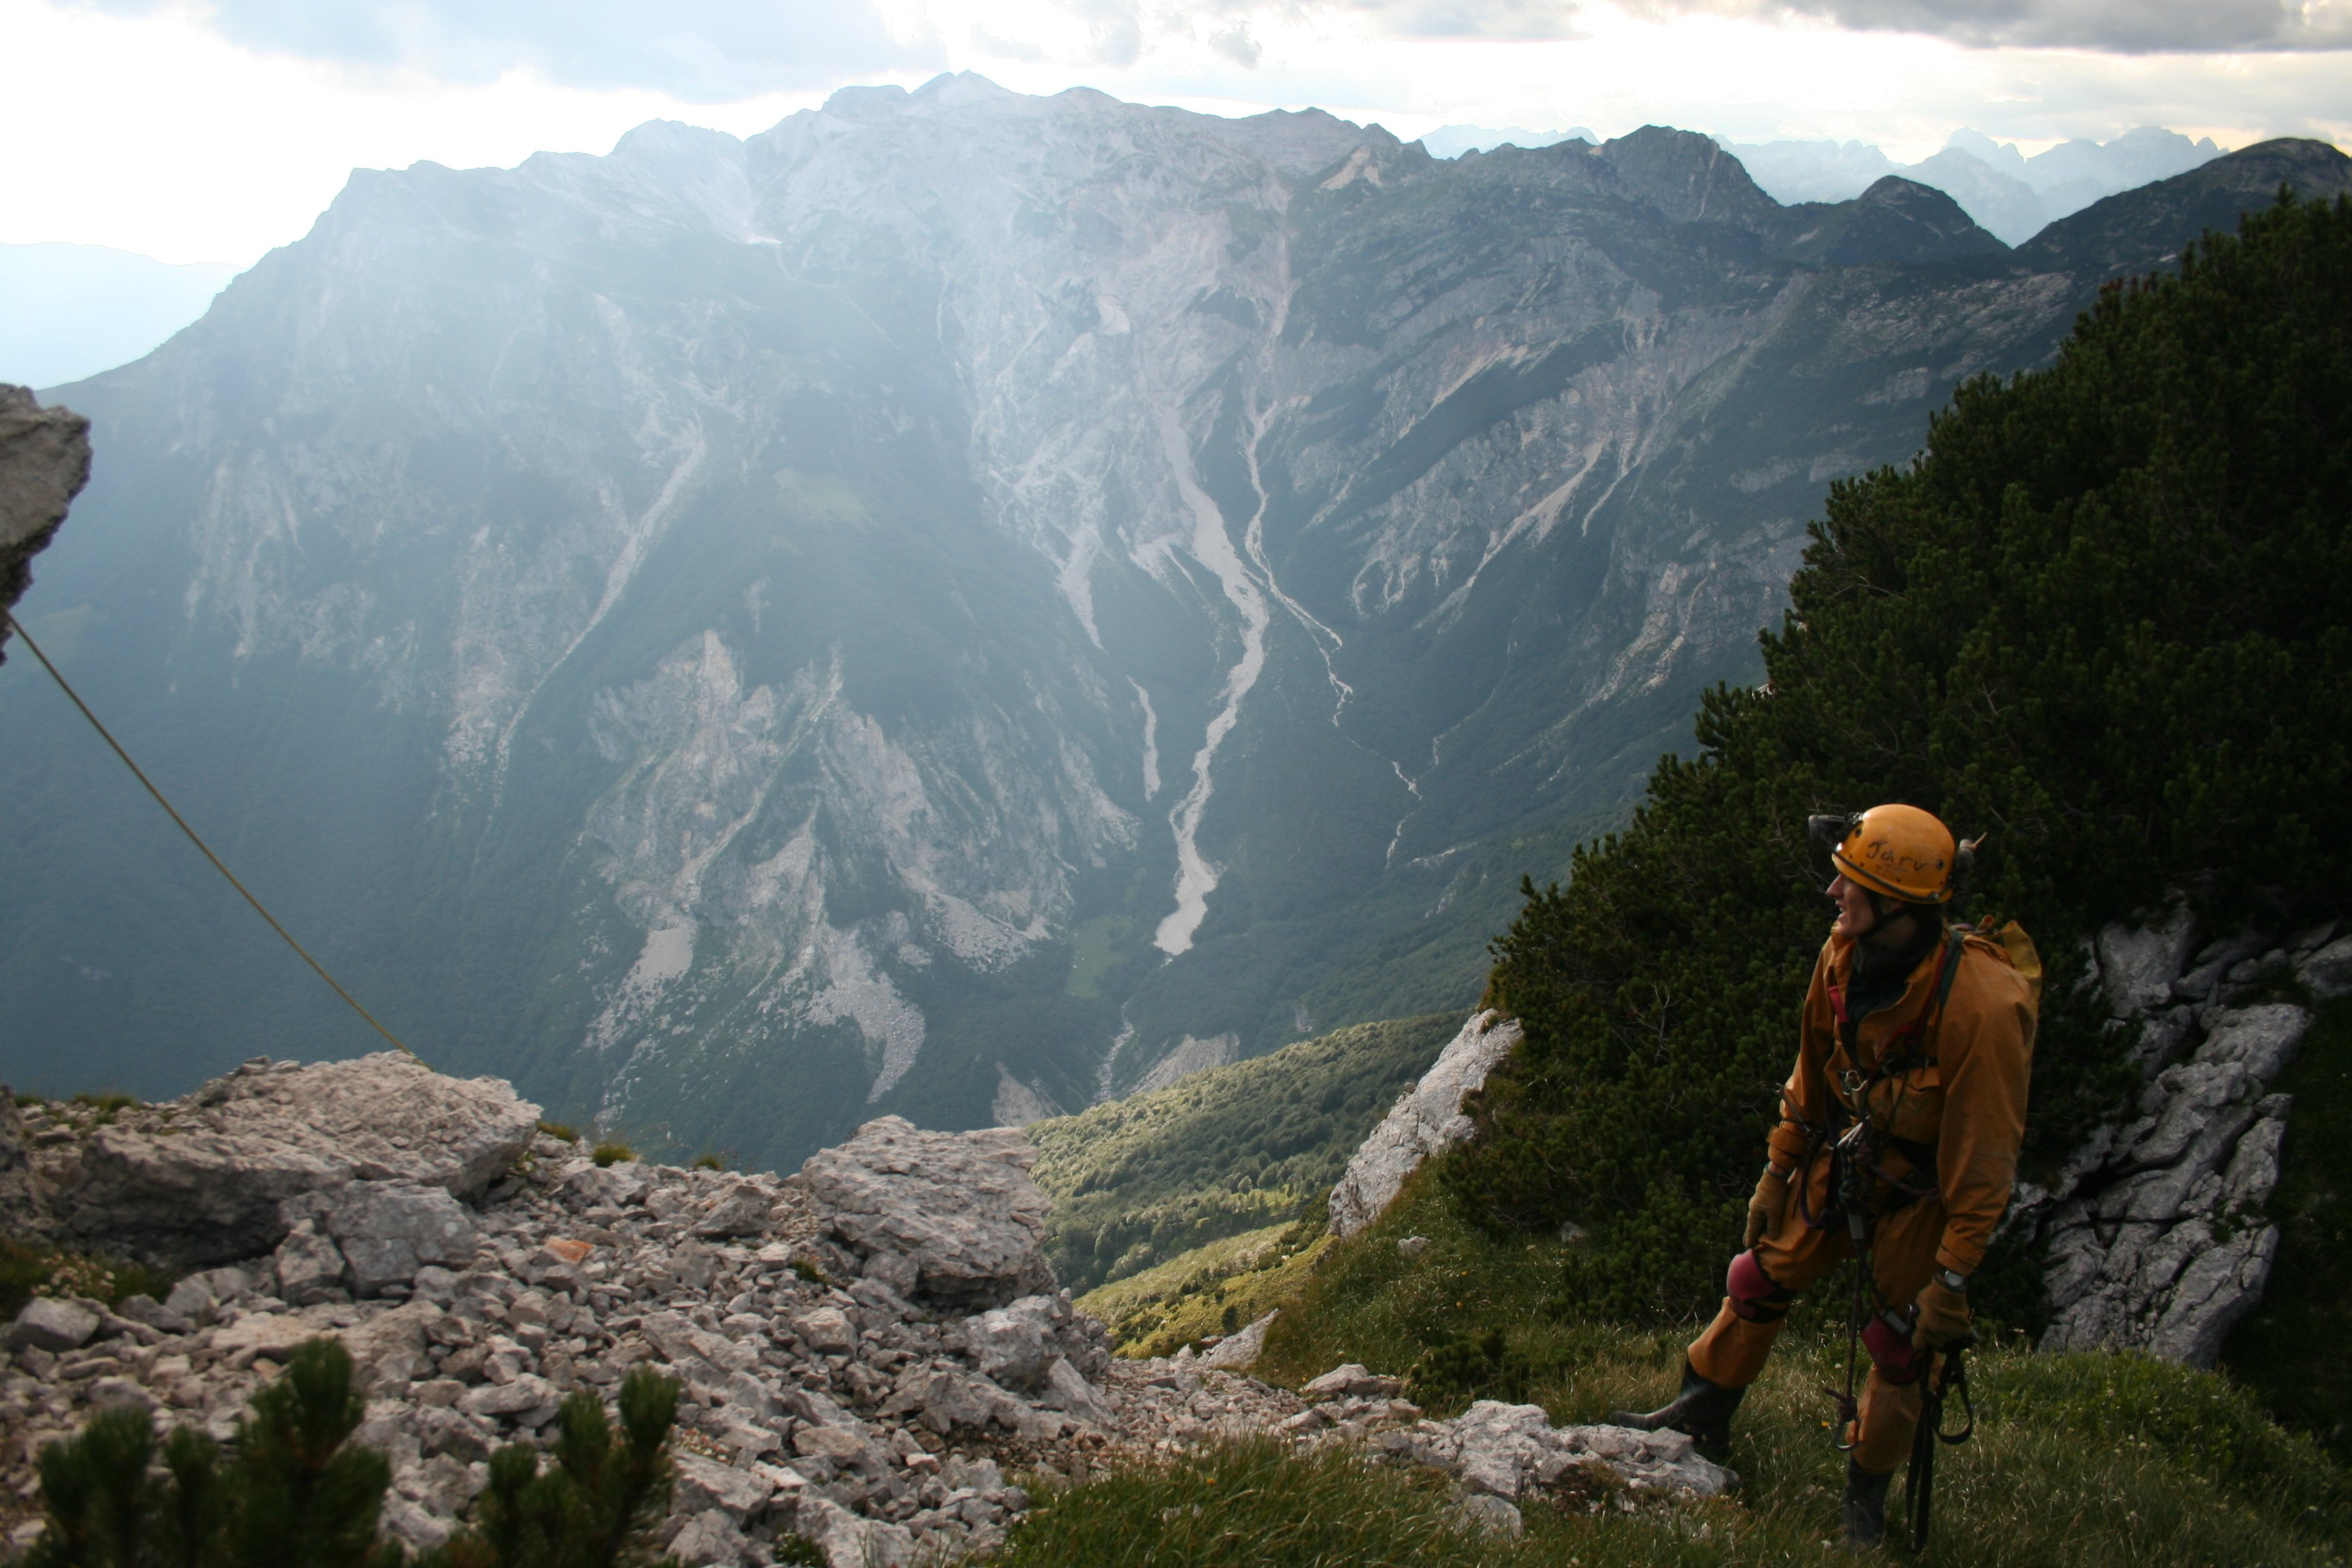
\includegraphics[width=0.99\textwidth]{2008/planika/Jana Carga - Canon 350D - img_3007 planika jama clifftop change--orig.jpg}}
\caption{Jarvist Frost stands at the top of the abseil to \protect\passage{Planika Jama}. \pic{Jana Čarga}}
\label{planika surface pitchead}
\end{pagefigure}

\clearpage

\subsection{29.07.08 - Hard Echo Rift push}

\margininbox{Planika Jama}{
     \begin{itemize}
    \item Jana Čarga
    \item Jarvist Frost
    \item Paul Hutton
    \end{itemize}}{\explo}

Straight to \passage{Echo Rift} \& started hammering (no lump, only bolt hammer).
4hrs later with Bob Dylan blaring, after a few tries with oversuit I
stripped to wet socks, furry \& safety hat (acrylic). I got my feet into
the chamber beyond up to my feet, but couldn't commit to not breathing
as I pushed past.

You know it's desperate when your wet socks freeze to the ground as you
get ready.

Problem is the S-bend nature of the rift. And my refusal to go
headfirst.

On way out, we derigged to first rebelay \& climbed into scary rift:
``\passage{Diggers of the U.G.}''. Loose boulders everywhere, above extension
Meander which forms lowest rebelay. BUT, off to the left is a strongly
blowing chamber through tight, but hammer-able, rift.

\name {Jarvist Frost}

\begin{figure*}
\checkoddpage \ifoddpage \forcerectofloat \else \forceversofloat \fi
\centering
    \begin{subfigure}{0.49\textwidth}
        \centering
        \frame{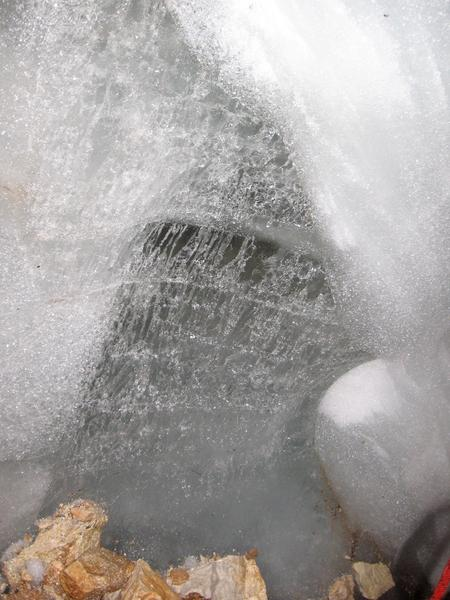
\includegraphics[width=\linewidth]{2008/planika/Jarvist Frost - canon a520 - planika - transparent ice in snow.jpg}} 
        \caption{} \label{ice planika}
    \end{subfigure}
        \hfill
\begin{subfigure}{0.49\textwidth}
\centering
\frame{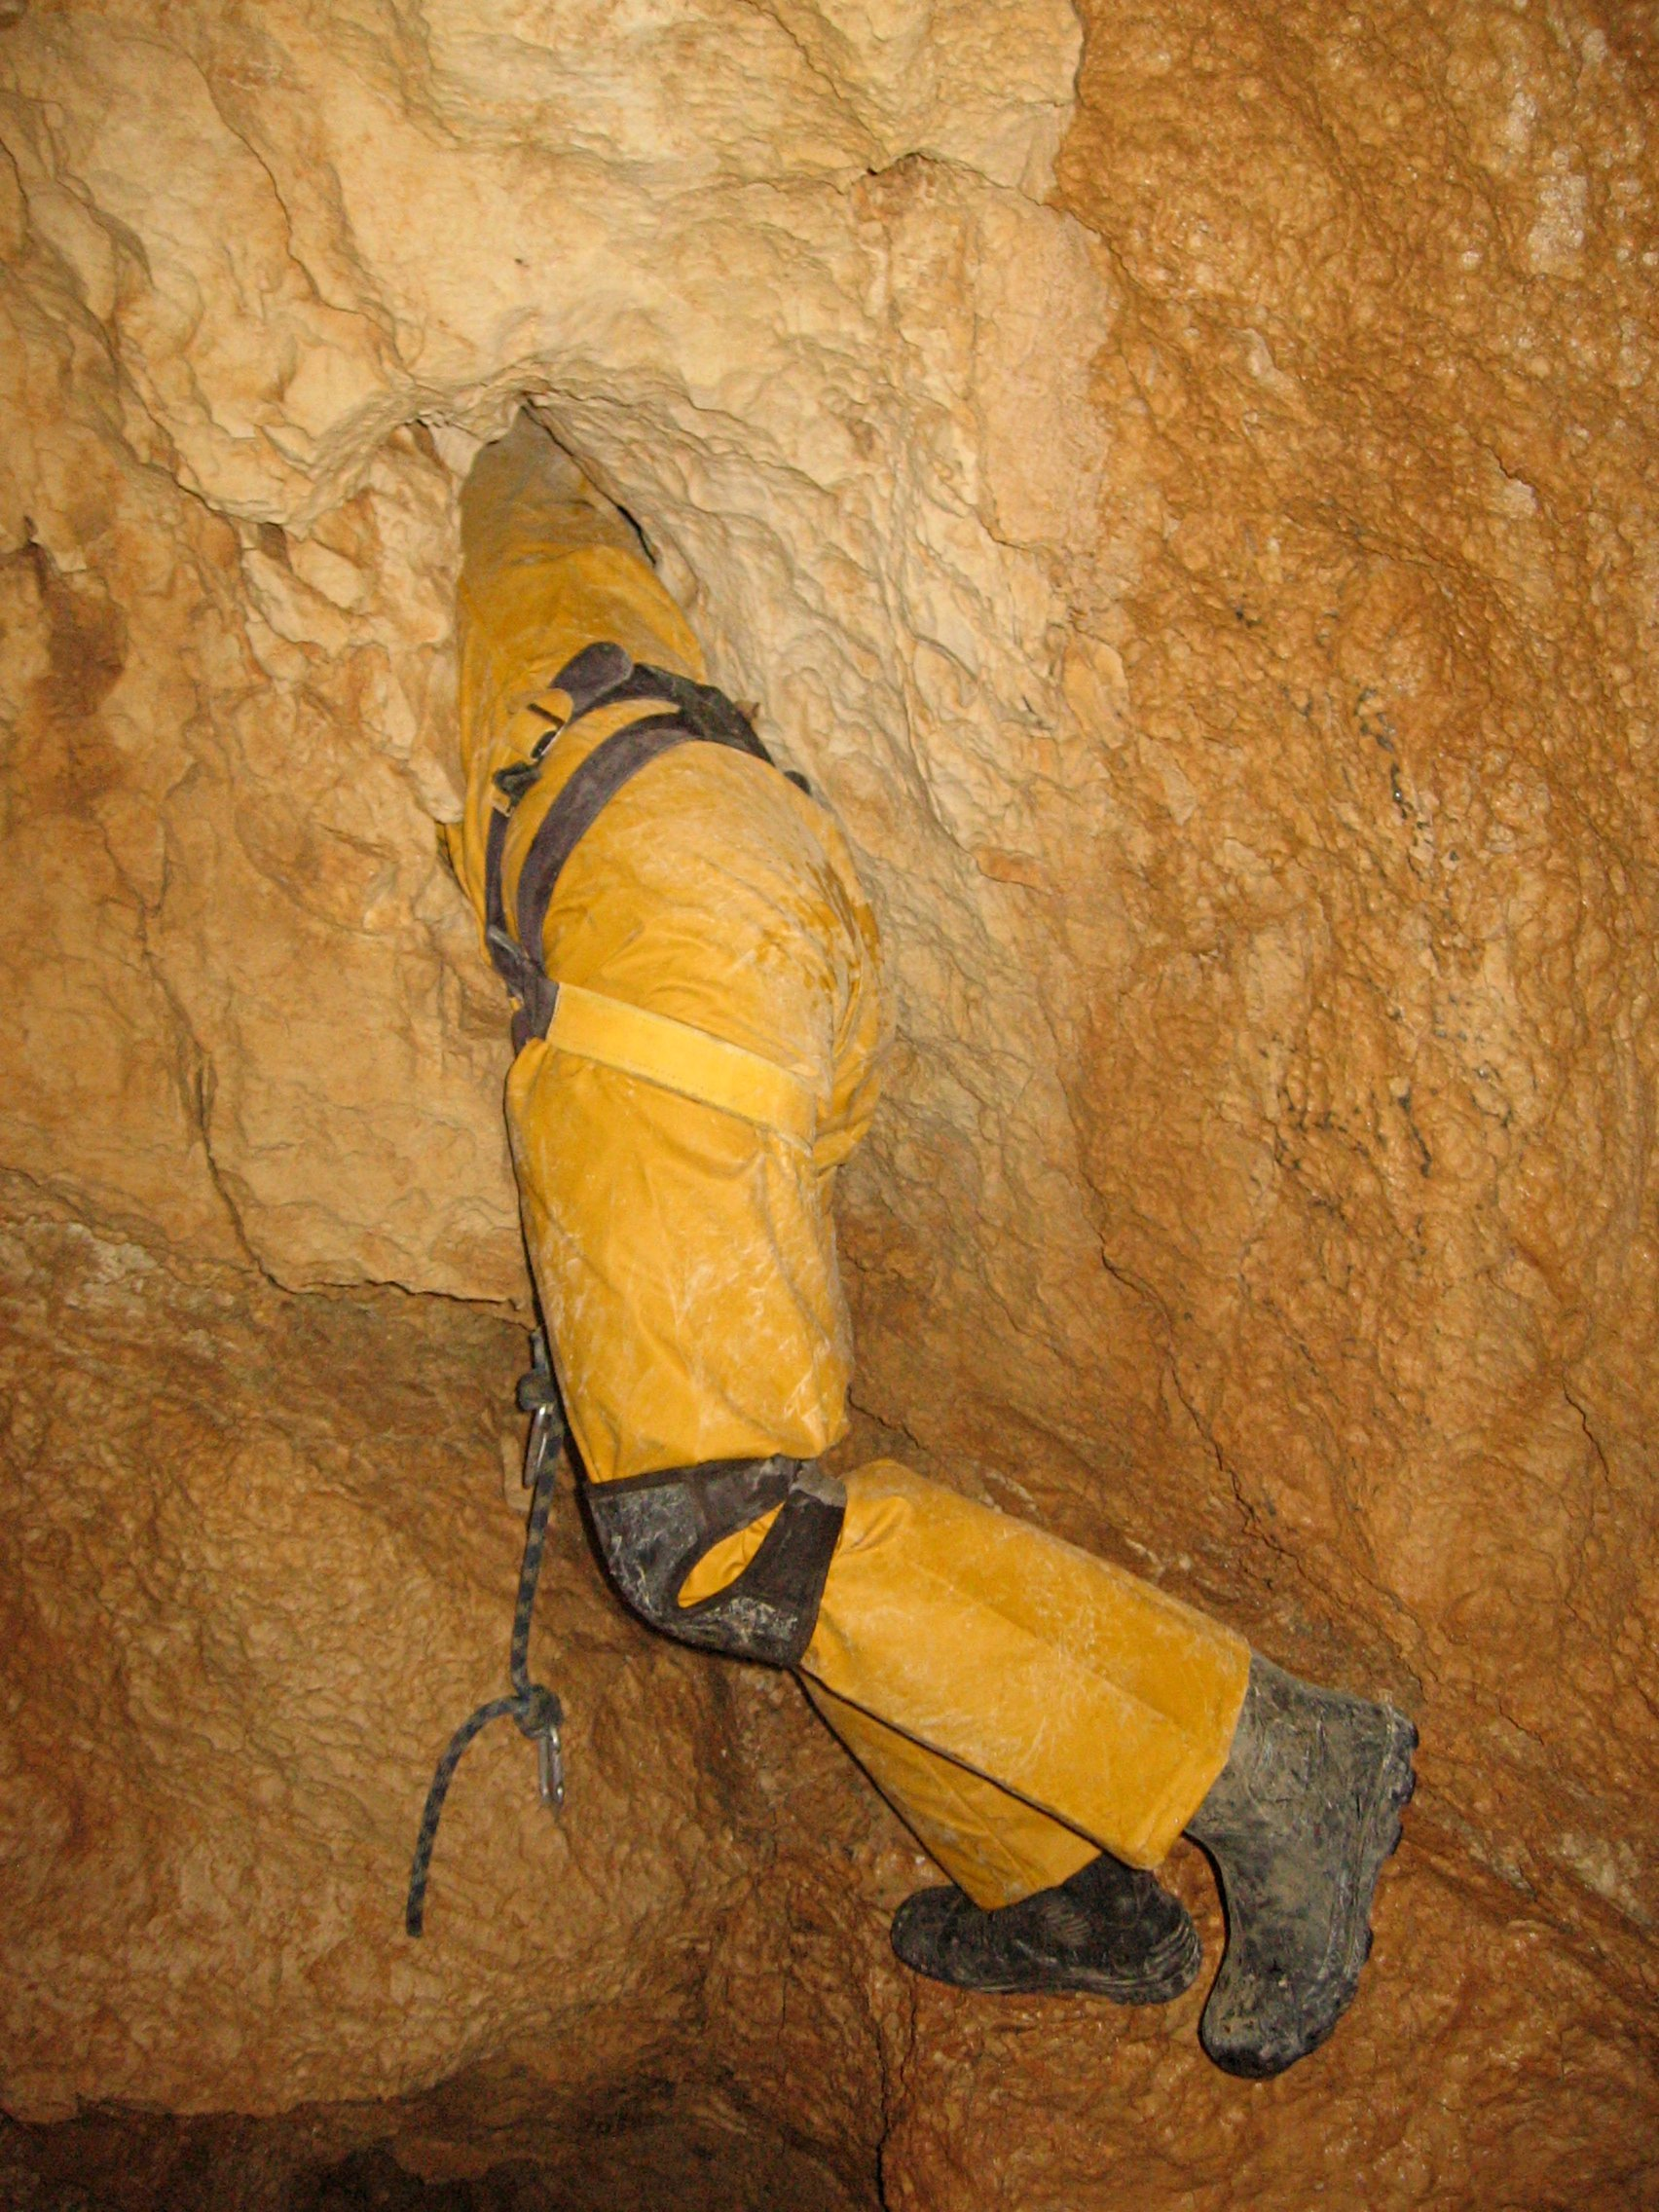
\includegraphics[width=\linewidth]{2008/planika/Jarvist Frost - canon a520 - planika - echo rift pushing front pre destruction--orig.jpg}}
 \caption{}\label{echo rift destruction}
\end{subfigure}

  \caption{\protect\passage{Planika Jama}. \emph{a}) Transparent ice within the snow. \emph{b}) Pushing in Echo Rift. \pic {Jarvist Frost}}
\end{figure*}
